\documentclass[12pt]{notes}

\usepackage{natbib}

% Command for Questions
%\question{}

% Command for Notes
% \note{}

% Code to create a minipage where you can type in class notes. 
%%\begin{minipage}[l][2cm][c]{\textwidth}
%\begin{comment}

%\end{comment}
%%\end{minipage}


% Begin Document
%==============================================================================
\begin{document}
% Include the Title of the Handout
\ntitle{D.2: Group Work Primer}

\section{How groups form}
% Include Numbered Sections
Understanding the \cite{tuckman1965} phases of group work, as summarized in \cite{cullen2015} (see Figure \ref{fig:group_stage}), helps to articulate how groups develop. 

\bi
\item Form
\bi
\item Desire for acceptance
\item Reliance of group leader
\item Largely superficial interactions
\ei
\item Storm
\bi
\item Competition and conflict among group members as task functions organize
\ei
\item Norm
\bi
\item Group members acknowledge contributions of others
\item Group cohesion develops
\ei
\item Perform
\bi
\item Group members truly interdependent on each other 
\item Group produces successful outcomes
\ei
\item Adjourn
\bi
\item Group member relationships end (in the group setting capacity anyway)
\ei
\ei

\question{How many of you have been in groups that never made it past the ``storm'' phase?}

\begin{minipage}[l][3cm][c]{\textwidth}

\end{minipage}

\question{Why do so many groups never make it to the ``perform'' stage?}

\begin{minipage}[l][3cm][c]{\textwidth}

\end{minipage}

\section{Potential Group Member Roles}
\bi
\item Fearless Leader
\bi
\item Assigns tasks (with the consent of the group) and organizes meetings
\item Makes sure the group keeps momentum through regular communication
\ei
\item Programmer Extraordinaire
\bi
\item Keeps track of all SAS (or other) code that group members write
\item Ensures that the submitted code is well documented (informative code comments), clean, and organized
\ei
\item Editor-in-Chief
\bi
\item Synthesizes the writing contributions of each member into a document with one, consistent voice
\item Should be the owner of the master file of the paper and be aware of all edits made to this file
\ei
\item Data Guru
\bi
\item Manages a copy of the master dataset
\item Understands the meaning of each variable
\item Ensures that the data description in the report and presentation are accurate
\ei
\item Articulate Ambassador
\bi
\item Conducts all communication with instructor regarding the project
\item Is the person in charge of turning in all group assignments
\ei
\ei

\section{Next Steps}
Each group should
\bi
\item Establish roles and expectations for each member
\item Decide when you will meet next (be aware of final project deadlines)
\item Decide on a group name and send this to Dr. Bean ASAP
\ei

\begin{figure}
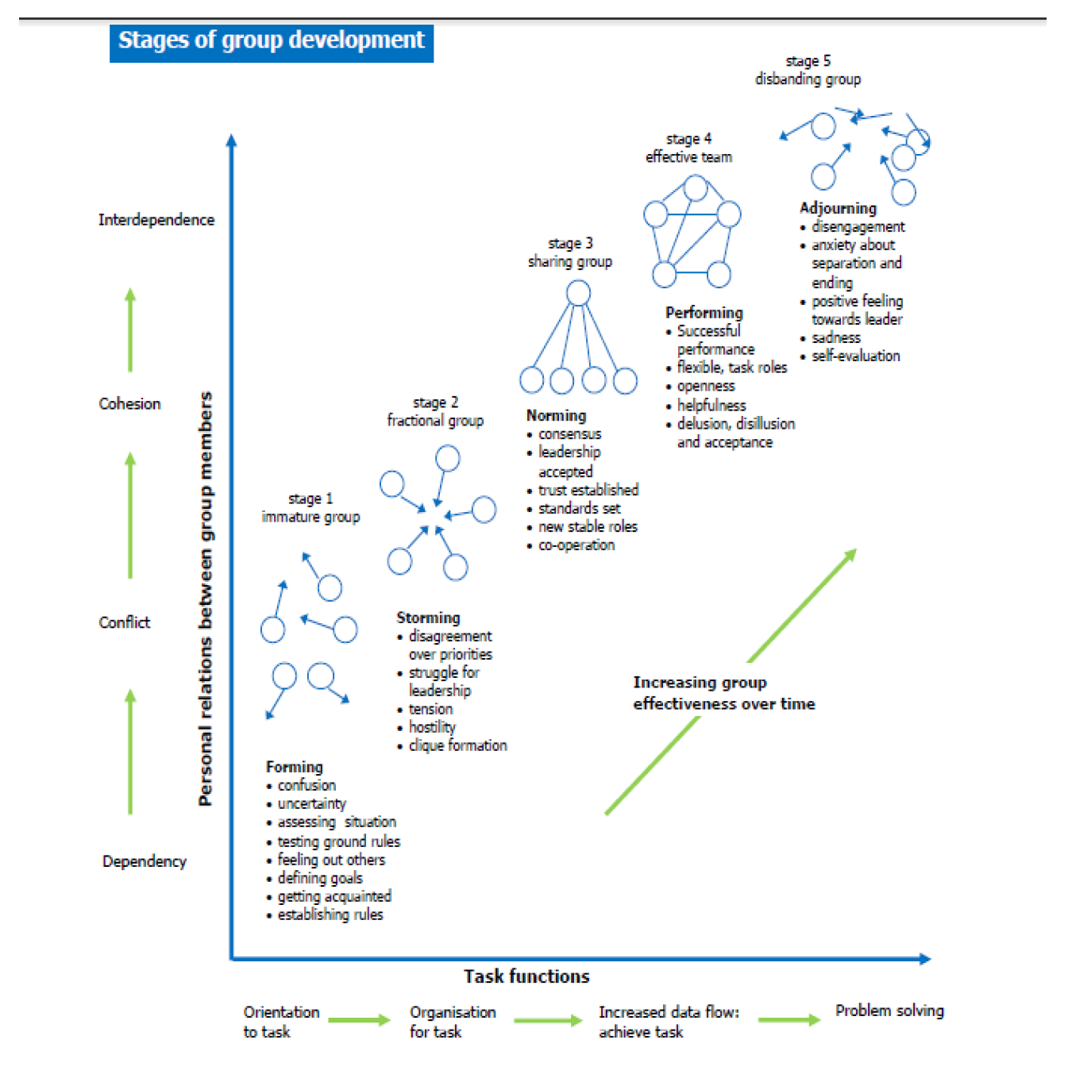
\includegraphics[width=\textwidth]{figures/moduleD/group_stages.png}
\caption{Tuckman's stages of group development (image taken from \cite{cullen2015}).}
\label{fig:group_stage}
\end{figure}




\bibliographystyle{apalike}
\bibliography{references}

% End the Document
%==============================================================================
\end{document}